\graphicspath{{./2-Arquitectura/capitulo4/}}

\Capitulo{Estrategia}{

En el complejo panorama empresarial actual, la definición y ejecución efectiva de estrategias se erige como un pilar fundamental para el éxito organizacional. La capa de estrategia en la arquitectura empresarial se presenta como un terreno fértil para la formulación y alineación de objetivos estratégicos, proporcionando un marco claro para la toma de decisiones que impulsan el crecimiento sostenible.

Este capitulo se sumerge en la capa de estrategia, aprovechando las herramientas robustas de ArchiMate. \textbf{Esta capa se convierte en el epicentro donde las metas de alto nivel, los principios rectores y las iniciativas estratégicas se entrelazan para dar forma al futuro de la organización.
}
A lo largo de este documento, exploraremos de manera detallada cada uno de los modelos dentro de la capa de estrategia. Desde la identificación de los \textbf{stakeholders} estratégicos hasta la formulación de \textbf{principios clave} y la especificación de las \textbf{metas estratégicas}, cada modelo desempeña un papel vital en la concreción de la visión organizacional.

El objetivo es proporcionar una visión integral y estructurada de la estrategia empresarial, utilizando los elementos gráficos y descriptivos de ArchiMate para comunicar eficazmente la complejidad inherente a la toma de decisiones estratégicas. Este análisis detallado, basado en las mejores prácticas de ADM, busca ser una guía esencial para buscar alinear la estrategia con la ejecución y lograr una ventaja competitiva sostenible.

Usaremos la Capa de Estrategia para descubrir cómo la arquitectura empresarial se convierte en un faro orientador para la toma de decisiones estratégicas en un entorno empresarial dinámico y desafiante.
}

%--------------Mapa de Capacidad-----------------------
\PuntoDeVista{Mapa de Capacidad}{imgs/MapadeCapacidadM.pdf}{
    El punto de vista de mapa de capacidad  representa una estructura conceptual que demuestra cómo los recursos y las capacidades se integran de manera sinérgica para alcanzar resultados estratégicos en una organización. 
}{imgs/MapadeRecursoC.pdf}{Este caso de mapa de capacidad se centra en mostrar cómo la gestión de tecnologías de la información (TI), la administración de recursos humanos y el uso de herramientas tecnológicas se entrelazan estratégicamente para alcanzar un nivel elevado de satisfacción con el producto final. Este enfoque integrador reconoce la importancia de \textbf{coordinar eficientemente los aspectos clave de la gestión, recursos y tecnologías en el proceso}, asegurando que la entrega del producto final no solo cumpla con los estándares requeridos, sino que también satisfaga las expectativas del usuario de manera óptima. }{0.5}{0.7}

%--------------Realización de Resultados-----------------------
\newpage
\section{Realización de Resultados}
\subsection{Modelo}
\begin{figure}[H]
	\centering	
    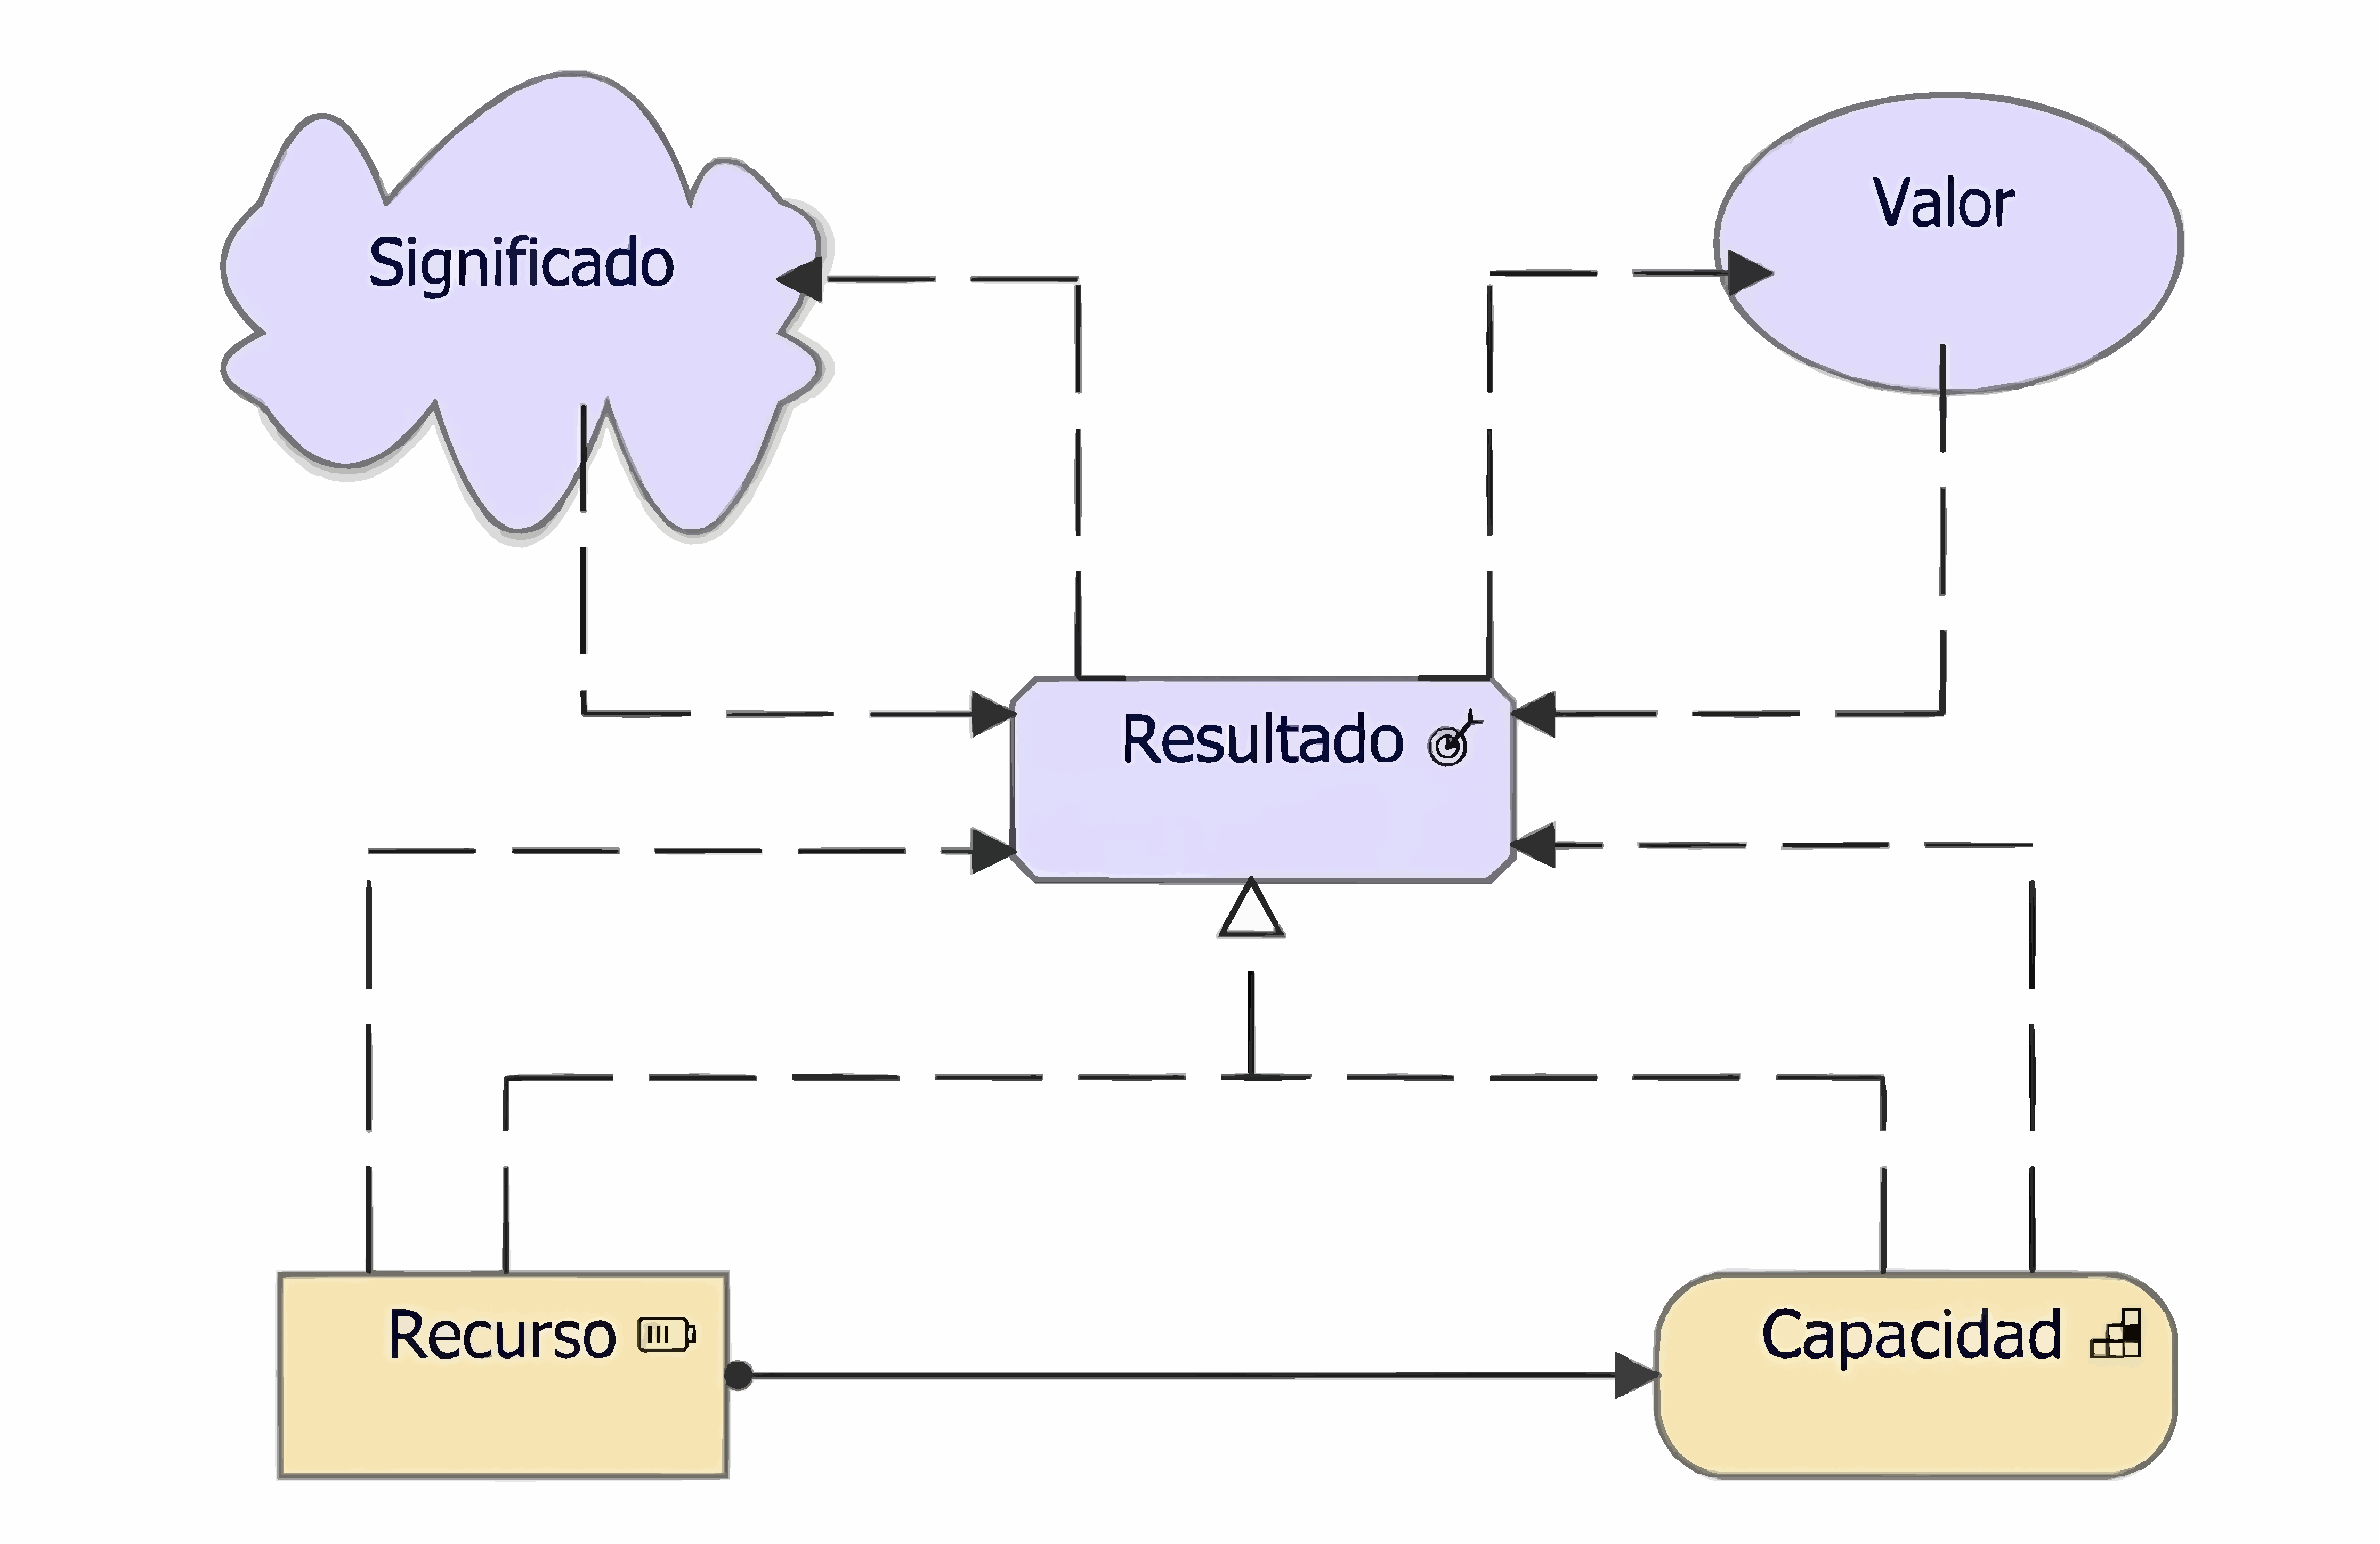
\includegraphics[width=0.7\linewidth]{imgs/RealizaciondeResultadoM.pdf}
	\caption{Modelo realización de resultados}
\end{figure}
El modelo de organización se utiliza para representar la estructura y relaciones internas de una entidad empresarial. Este modelo ayuda a entender cómo se organizan y se relacionan los diferentes roles, actores y colaboraciones dentro de la empresa. Estos elementos se interconectan para formar la estructura organizativa que soporta la arquitectura de negocio.
\subsection{Caso}
\begin{figure}[H]
	\centering	
    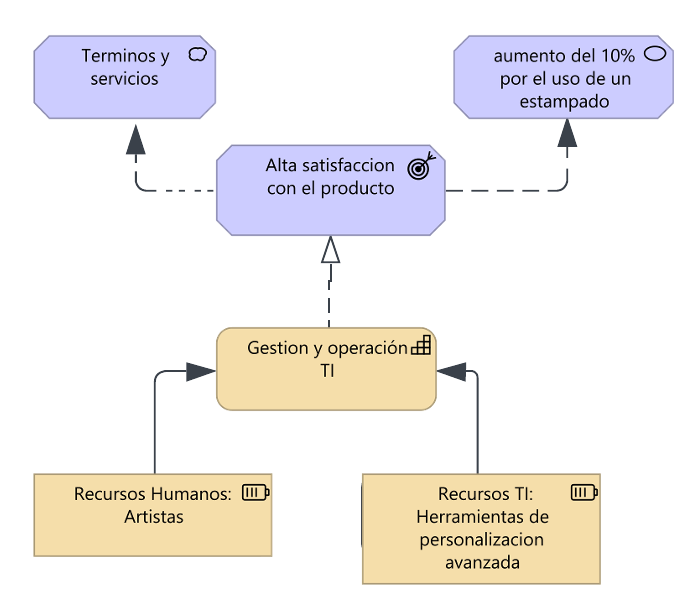
\includegraphics[width=0.7\linewidth]{imgs/Caso 2.png}
	\caption{Caso realización de resultados}	
 \end{figure}
Este caso proporciona una representación visual esclarecedora de la correlación directa entre la calidad de los términos y servicios ofrecidos y el nivel de satisfacción del cliente alcanzado. Este último no solo se logra a través de la entrega de productos o servicios, sino también mediante una \textbf{gestión eficiente y una operación óptima de las tecnologías de la información (TI).}

%--------------Mapa de Recurso-----------------------
\PuntoDeVista{Mapa de Recurso}{imgs/MapadeRecursosM.pdf}{
    Este modelo visualiza cómo los recursos se relacionan con las capacidades en el contexto de la estrategia organizacional. Es una herramienta útil para planificar y gestionar los recursos necesarios para lograr los objetivos estratégicos.
}{imgs/MapadeCapacidadC.pdf}{En este caso el mapa de recurso representa la integración de recursos humanos y tecnológicos con el objetivo de lograr la exitosa construcción de una tienda virtual. Este visual proporciona una herramienta valiosa para la planificación y gestión de proyectos, destacando la colaboración eficiente entre el personal y las tecnologías necesarias. Permitiendo una coordinación efectiva y la maximización de los recursos para alcanzar el éxito en el proyecto.}{0.6}{0.7}



%------------Flujo de Valor-------------------------
\section{Flujo de valor}
\subsection{Modelo}
\begin{figure}[H]
	\centering	
    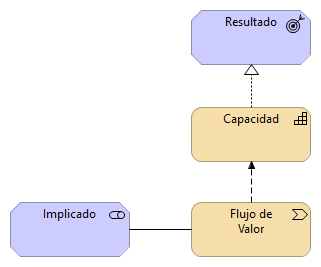
\includegraphics[width=0.55\linewidth]{imgs/FlujodeValorM.png}
	\caption{Modelo flujo de valor}
\end{figure}
La perspectiva del flujo de valor involucra la interrelación entre recursos y actividades con el propósito de generar valor en el marco de la estrategia organizacional. Proporciona una visión integral que facilita la planificación estratégica y la toma de decisiones, permitiendo una gestión más eficaz de los recursos y una optimización de las actividades para impulsar el valor añadido a la organización.
\subsection{Caso}
\begin{figure}[H]
	\centering	
    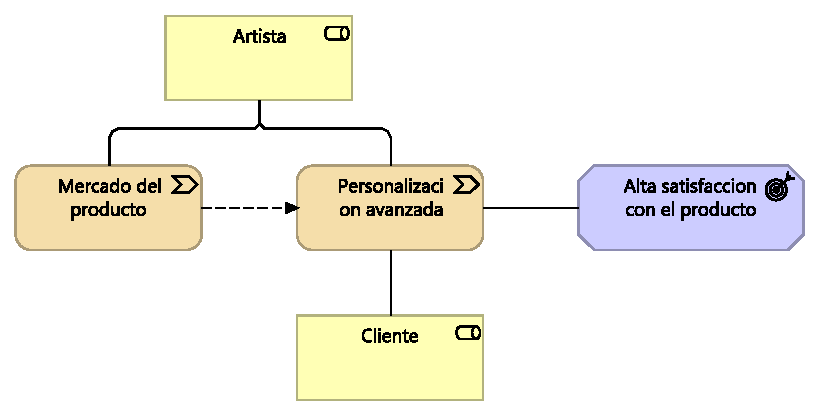
\includegraphics[width=0.9\linewidth]{imgs/Caso 4.pdf}
	\caption{Caso flujo de valor}	
 \end{figure}
 
El flujo de valor comienza con la creatividad del artista, convirtiendo ideas e innovación en diseños con gran potencial. Este proceso se encuentra con las necesidades del consumidor en el mercado, donde la personalización avanzada crea conexiones emocionales más profundas. \textbf{Esta interacción es clave para el éxito empresarial al garantizar la relevancia y competitividad de las camisetas.} Este flujo culmina en la satisfacción del cliente, superando expectativas y generando lealtad, impulsando el crecimiento y la reputación de la marca.

%----------------------Estrategia----------------------
\PuntoDeVistaResponsive{Estrategia}{imgs/EstrategiaM.pdf}
{
  El modelo de estrategia es fundamental para planificar y alinear las iniciativas estratégicas con los recursos y capacidades de la organización. Estos elementos se interrelacionan para formar una visión cohesiva de cómo la estrategia se traduce en acción. Este modelo se utiliza para asegurar que la estrategia de negocio se integra adecuadamente con la arquitectura empresarial.

}
{imgs/Caso 5.pdf}
{
Estos elementos, respaldados por políticas empresariales sólidas y una estrategia efectiva de desarrollo del marketing, son la base para alcanzar los objetivos específicos y adherirnos a los principios de la marca. La integración de recursos humanos, TI y económicos es fundamental para implementar esta estrategia y lograr rentabilidad y crecimiento sostenible. En el núcleo del modelo “Estampa tu idea”, una plataforma web donde los usuarios pueden personalizar completamente sus camisetas, y donde los diseñadores  y artistas pueden colaborar creativamente. \textbf{Esta plataforma es el corazón de nuestra propuesta de valor y será el medio para conectar con nuestra audiencia y ofrecer un producto verdaderamente único.}
}{0.9}{1.1}